\section{Trasduttore elettromagnetico}
Esso è realizzato da un solenoide entro il quale viene inserito un
magnete permanente. Il magnete effettua un movimento all'interno del
solenoide; da questo movimento sappiamo ricavare la velocità
calcolando la derivata dello spostamento effettuato nel tempo.

%figura

Come per il trasformatore differenziale \ref{sec:trasdiff},
calcoliamo il flusso del campo magnetico all'interno delle spire
coperte dal magnete. La variazione del flusso ci indica lo
spostamento del magnete, e quindi derivando questa quantità rispetto
al tempo, otteniamo la velocità:

	\[V=-\frac{d(N_c\phi_B)}{dt}= -n\phi_B\frac{dx}{dt}
	   =-n\phi_B v\]


\section{Dinamo tachimetrica}
Il rotore è fisicamente costituito da un materiale ad elevatissima
permeabilità magnetica su cui è avvolto ad elica un filo chiuso su sé
stesso e connesso in punti situati ad intervalli regolari.
Sui segmenti del collettore sono poste delle spazzole su cui striscia
il rotore, queste poi sono collegate ai morsetti della macchina.

\begin{figure}[htbp]
	\centering
	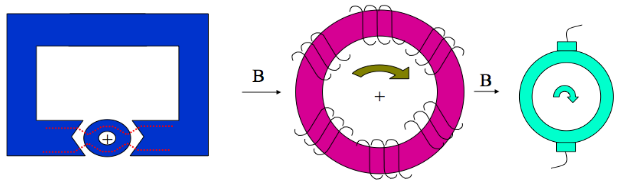
\includegraphics[scale=0.5]
			{img/dinamo.png}
	\caption{Struttura di una dinamo tachimetrica
\label{fig:dianmo}}
\end{figure}

Il rotore ruota in un campo magnetico generato da un magnete
permanente. Essendo il rotore ad alta permeabilità magnetica, tutte le
linee di forza del campo magnetico B, che partono dai poli del
magnete, si concentrano entro il rotore. Posizionando le spazzole
nella parte alta e nella parte bassa riusciamo a ricavare una forza
elettro motrice non nulla che ci può indicare la velocità di
rotazione. Consideriamo la tensione fornita da una singola spira:

	\[e = \overrightarrow{v} \wedge \overrightarrow{B} \times
\overrightarrow{L} \]

dove $\overrightarrow{v}$ è la velocità tangenziale del rotore,
$\overrightarrow{B}$ il campo magnetico e $\overrightarrow{L}$ lo
spessore del rotore. Ne consegue che il contributo di una singola
spira soggetta al campo magnetico $B$ è:

	\[e=vBL\]

Data la simmetria del rotore la somma delle f.e.m. indotte è nulla;
l'uso delle spazzole però consente di ottenere una f.e.m. non nulla
in quanto divide in due rami il rotore. La situazione è
modellabile come due serie di generatori di tensione messi in
parallelo. Ne risulta che la f.e.m. indotta totale è:

	\[E=e_{medio}\frac{N}{2}= vB_{medio}L\frac{N}{2}\]

dove $N$ è il numero totale di spire. Ricaviamo ora il valore della
f.e.m. in funzione del numero di giri del rotore:

	\[\phi_B=\int BdS=B_{medio}S=L\pi r B_m \]
	\[E=v\frac{\phi_B}{L \pi r}L\frac{N}{2}\]

Sappiamo che $v=\omega r= 2\pi n r$ dove $n$ è il numero di giri al
secondo, quindi possiamo scrivere:

	\[E=\phi_B n N\]

La f.e.m. indotta nella bobina è sempre sinusoidale se il campo B è
uniforme, ma ogni volta che il flusso concatenato è massimo (e quindi
la f.e.m. indotta ha il valore zero) il contatto s'inverte, in modo
che ogni spazzola è sempre in contatto con un semi-anello che ha la
stessa polarità. Con questo la tensione fra le spazzole, e quindi fra
i morsetti A e B della macchina, ha sempre il medesimo segno.
Aumentando il numero di spire, la tensione che ne risulta è pressapoco
continua, questo però non impedisce l'ondulazione (cioè il passaggio
fra un elettrodo e un altro). Con la dinamo tachimetrica purtroppo non
è possibile utilizzare dei filtri per eliminare il rumore dato che
questo dipende dalla velocità con cui si muove il rotore.

\section{Alternatori tachimetrici}
Un trasduttore di questo tipo è costituito da un magnete rotante che
genera tensioni alternata su degli avvolgimenti fissi.

\begin{figure}[htbp]
	\centering
	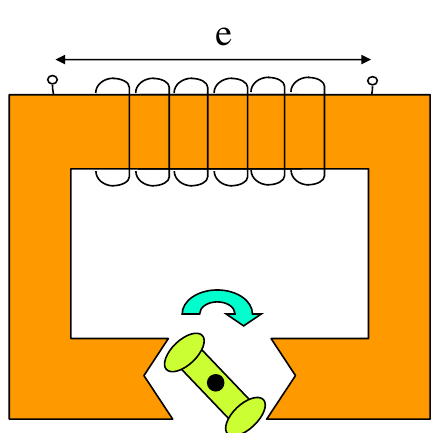
\includegraphics[scale=0.5]
			{img/alternatoretachi.png}
	\caption{Alternatore tachimetrico\label{fig:altachi}}
\end{figure}


La frequenza e l'ampiezza della tensione alternata rilevata sono
proporzionali alla velocità di rotazione. La misura della velocità è
ricavabile da entrambe le variabili.

%FIXME conti

\section{Generatori ad induzione}

%FIXME da fare

\section{Trasduttore a carica e scarica capacitiva}
Si tratta di un collettore rotante a quattro segmenti con quattro
elettrodi fissi. Due dei segmenti sono collegati assieme per mezzo di
un condensatore. Due elettrodi sono alimentati e i rimanenti due sono
collegati ad un carico.

\begin{figure}[htbp]
	\centering
	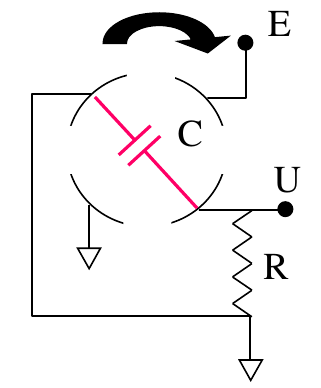
\includegraphics[scale=0.5]
			{img/caricascaricacapacitiva.png}
	\caption{Trasduttore a carica e scarica capacitiva
\label{fig:carscarcap}}
\end{figure}

Durante la rotazione il condensatore si carica quando i due segmenti
toccano gli elettrodi alimentati, mentre si scarica quando tocca gli
elettrodi con il carico. La velocità di rotazione viene determinata
attraverso la frequenza degli impulsi di carico del condensatore
rilevati sul ramo a cui è collegato il carico ($U$). Questa misura è
ottenibile mediante l'uso di un frequenzimetro. In alternativa al
frequenzimetro è possibile utilizzare l'integratore approssimato
mostrato in figura \ref{fig:carscarint}:

\begin{figure}[htbp]
	\centering
	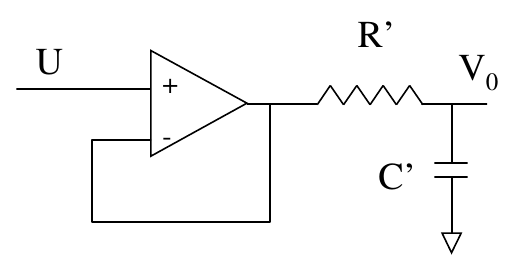
\includegraphics[scale=0.5]
			{img/caricascaricaintegra.png}
	\caption{Integratore approssimato per la rilevazione della
frequenza
\label{fig:carscarint}}
\end{figure}

Ponendo $R'C' >> \frac{T}{2}$ otterremo che il valore della tensione
in uscita $V_o$ corrisponderà al valore medio della tensione in
uscita sul trasduttore:

	\[ V_o = 2ERC\frac{1}{T} = 2fERC \]

Ovviamente la velocità di rotazione ha un limite superiore dovuto al
tempo di carico/scarico del condensatore. Inoltre nel caso
dell'integratore approssimato, la precisione diminuisce vicino a
questo limite. Un frequenzimetro garantisce una migliore precisione.

\section{Trasduttore elettro-ottico}
Con l'ausilio di un traduttore encoder e un'opportuna logica è
possibile calcolare la angolare oltre che il senso di rotazione.